\tikzstyle{rednode}=[circle, fill=red!50, minimum size=1.5]
\tikzstyle{line}=[line width=1]
\tikzstyle{node}=[midway, font=\footnotesize]
\newcommand{\drawmwpmgrid}{
  \draw[step=.4cm, opacity=.25] (-.4,-.4) grid (4.4,4.4);
  \draw (-.4,-.4) rectangle (4.4,4.4);
  \node[rednode] (1) at (0.5,0.4)  {};
  \node[rednode] (2) at (2,0.7)    {};
  \node[rednode] (3) at (2.5,1.2)  {};
  \node[rednode] (4) at (4,1)      {};
  \node[rednode] (5) at (0.75,2.1) {};
  \node[rednode] (6) at (1.95,2.4) {};
  \node[rednode] (7) at (1.6, 3.4) {};
  \node[rednode] (8) at (2.7, 3.5) {};
}
\begin{figure}[htbp]
    \centering
    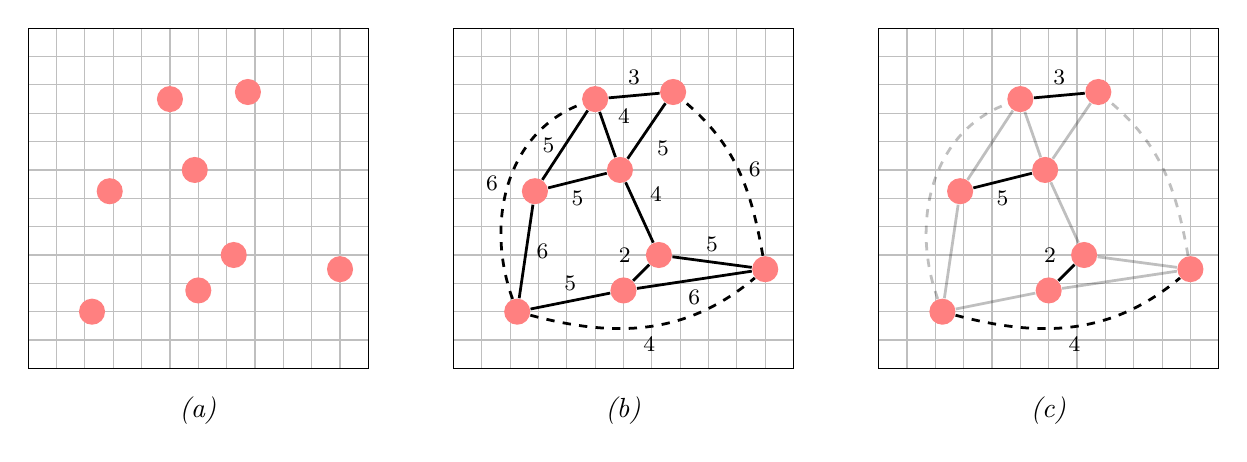
\begin{tikzpicture}[scale=0.9]
      \drawmwpmgrid
      \node at (2,-1) {\emph{(a)}};
    
      \begin{scope}[shift={(6,0)}]
        \drawmwpmgrid
        \draw[line] (2) -- (1) node[node,above]{5} -- (5) node[node, right]{6} -- (6) node[node, below]{5} -- (7) node[node, above right]{4} -- (8) node[node, above]{3} -- (6) node[node, below right]{5};
        \draw[line] (2) -- (3) node[node, above left]{2} -- (4) node[node, above]{5} -- (2) node[node, below]{6};
        \draw[line] (6) -- (3) node[node,above right]{4};
        \draw[line] (5) -- (7) node[node, left]{5};
        \draw[line, dashed] (1) to [out=-15, in=220] node[node,below]{4} (4);
        \draw[line, dashed] (4) to [out=100, in=-40] node[node,right]{6} (8);
        \draw[line, dashed] (1) to [out=110, in=200] node[node,left]{6} (7);
        \node at (2,-1) {\emph{(b)}};

      \end{scope}
      
      \begin{scope}[shift={(12,0)}]
        \drawmwpmgrid
        \draw[line, opacity=.25] (6) -- (3) -- (4) -- (2) -- (1);
        \draw[line, opacity=.25] (1) -- (5) -- (7) -- (6) -- (8) ;
        \draw[line] (7) -- (8) node[node, above]{3};
        \draw[line] (5) -- (6) node[node, below]{5};
        \draw[line] (2) -- (3) node[node, above left]{2};
        \draw[line, dashed] (1) to [out=-15, in=220] node[node,below]{4} (4);
        \draw[line, dashed, opacity=.25] (4) to [out=100, in=-40] (8);
        \draw[line, dashed, opacity=.25] (1) to [out=110, in=200] (7);
        \node at (2,-1) {\emph{(c)}};

      \end{scope}
    \end{tikzpicture}
    \caption{Visualizing the graph matching problem of minimum-weight pairs between anyons. (a) The set of anyons from the measured syndrome are the nodes in the graph matching problem. (b) The graph is initiated by connecting all nodes in the graph with edges weighted correspondingly to the shortest distance between the anyons. High-weight edges have been excluded here for clarity. (c) The minimum-weight subset of edges is the result. This figure is inspired by others \cite{naomi2016thesis}.}\label{fig:mwpm}
  \end{figure}
  